\documentclass[10pt,a4paper]{article}
\usepackage[left=2cm,right=2cm,top=2cm,bottom=2cm]{geometry}
\usepackage[dvipsnames]{xcolor}
\usepackage[fleqn]{mathtools}
\usepackage{booktabs}
\usepackage{amsmath}
\usepackage{latexsym}
\usepackage{graphicx}
\usepackage{nccmath}
\usepackage{multicol}
\usepackage{listings}
\usepackage{tasks}
\usepackage{color}
\usepackage{float}
\usepackage{lipsum}

\definecolor{colorIPN}{rgb}{0.5, 0.0,0.13}
\definecolor{colorESCOM}{rgb}{0.0, 0.5,1.0}
\graphicspath{ {imagenes/} }

\begin{document}
%#########################################################
\begin{titlepage}
	\centering
	{ \huge \bfseries \color{colorIPN}{Instituto Politécnico Nacional} \par}
	{ \Large \bfseries  \color{colorESCOM}{Escuela Superior de Cómputo} \par }
	\vspace{1cm}
	{\huge\Large \color{colorIPN}{Tecnologías para Desarrollo de Aplicaciones Web}.\par}
	\vspace{1.5cm}
	{\huge\Large  \color{colorESCOM}{Avance del Proyecto: Aplicación Web para reporte de ventas de una tienda de conveniencia}\par}
		\vspace{2cm}
	{\Large\itshape \color{colorIPN}{Profesor: M. en C. José Asunción Enríquez Zárate}\par} \hfill \break
	{\Large\itshape \color{colorIPN}{Alumnos:}\par} \hfill \break
	{\Large\itshape \color{colorIPN}{Hurtado Morales Emiliano}\par} \hfill \break
	{\Large\itshape \color{colorIPN}{Martínez Armando}\par} \hfill \break
	{\Large\itshape \color{colorIPN}{Aguirre Cassandra}\par} \hfill \break
	\vspace{1cm}
	{\Large\itshape \color{colorIPN}{Hernández Bryan}\par} \hfill \break
	{\Large\itshape \color{colorIPN}{ehurtadom1700@alumno.ipn.mx}\par} \hfill \break
	{\Large\itshape \color{colorIPN}{@alumno.ipn.mx}\par} \hfill \break
	{\Large\itshape \color{colorIPN}{@alumno.ipn.mx}\par} \hfill \break
	{\Large\itshape \color{colorIPN}{@alumno.ipn.mx}\par} \hfill \break
	{\Large\itshape \color{colorIPN}{4CM3} \par}
	\vfill
	{\large \color{colorIPN}{\today}\par} 
	\vfill
\end{titlepage}

\renewcommand\lstlistingname{Quelltext} 

\lstset{ 
	language=Java,
	basicstyle=\small\sffamily,
	numbers=left,
	numberstyle=\tiny,
	frame=tb,
	tabsize=4,
	columns=fixed,
	showstringspaces=false,
	showtabs=false,
	keepspaces,
	commentstyle=\color{Violet},
	keywordstyle=\color{colorIPN} \bfseries,
	stringstyle=\color{colorESCOM}
}

\settasks{
	counter-format=(tsk[r]),
	label-width=4ex
}

\tableofcontents 
\pagebreak

\listoffigures
\pagebreak

%################################################
\section{\color{colorIPN}{Introducción}}
El reporte de ventas es un informe donde se recogen las actividades comerciales de una empresa. Su objetivo es evaluar el desempeño del departamento comercial, las estrategias de ventas y el trabajo de los representantes, para  identificar fallas y oportunidades de mejora en los procesos. 

La función principal del departamento comercial es atraer clientes, vender más y de forma más eficiente. El reporte de ventas es la herramienta que permite reunir y analizar el volumen de ventas de la empresa, determinar la efectividad de las acciones que realizas para generar ventas y evaluar la productividad de los agentes de ventas.

\subsection{ \color{colorESCOM}{Modelo E-R}}
Un modelo de entidad relación (modelo E-R) es el diseño de la estructura lógica de una base de datos, que luego se podrá implementar como una base de datos real. Los componentes principales del modelo E-R son un conjunto de entidades y de relaciones.

Un modelo de entidad relación describe cosas de interés interrelacionadas en un dominio específico de conocimiento. En ingeniería de software, el modelo E-R se utiliza generalmente para incorporar cosas que necesita recordar una empresa para efectuar los procesos empresariales.

\subsection{ \color{colorESCOM}{Modelo Relacional}}
Un modelo relacional consiste en representar datos por medio de tablas relacionadas cuyas filas se llaman tuplas y las columnas variables, conformando así una base de datos.

Existen una serie de términos formales que se corresponden con expresiones informales.

\begin{itemize}
	\item La relación, que es el término formal, tiene en la tabla su equivalente informal.
	\item La tupla no es más que un registro que se representa en las filas de la tabla y el atributo es una columna o campo.
	\item La cardinalidad se refiere al número de filas o registros y el grado es el número de columnas o campos.
	\item Por último, la clave primaria es un identificador único de cada caso.
\end{itemize}

\subsection{ \color{colorESCOM}{Diccionario de Datos}}
Un diccionario de datos trata de documentar los metadatos más ligados a su almacenamiento en la base de datos. Es decir, incluye aspectos técnicos como el tipo de dato, formato, longitud, posibles valores que puede tomar e, incluso, transformaciones sufridas, sin olvidar la definición de cada campo. 

La documentación de estas transformaciones proporciona automáticamente el linaje del dato, entendido como la trazabilidad a lo largo de su ciclo de vida. Estos metadatos ayudan a los usuarios a entender los datos desde el punto de vista técnico para poder explotarlos adecuadamente. Por este motivo, cada base de datos debería contar con su diccionario de datos asociado. 
\pagebreak

%################################################
\section{\color{colorIPN}{Conceptos}}

\begin{itemize}
	\item  Entidad: Cualquier cosa en la empresa que se representará en la base de datos.
	\item  Atributo: Describe la propiedad de una entidad.
	\item  Atributo Clave: Identifica de forma exclusiva una entidad de un conjunto de entidades.
	\item Relación: Muestra cómo se relacionan las entidades entre sí.
	\item Cardinalidad: Especifica cuántas instancias de una entidad se relacionan con una instancia de otra entidad.
	\item Tabla: Herramienta de organización de información que se utiliza en bases de datos en la informática.
	
\end{itemize}

\pagebreak

%################################################
\section{\color{colorIPN}{Desarrollo}}
En este apartado, se presenta la estructura general de la base de datos del proyecto Registro de Venta, mediante esta estructura se puede visualizar la manera en que se relacionan todos los elementos de la base de datos y los paquetes en los que se dividió la base de datos.

%################################################
\subsection{
	\textit{
		\color{colorESCOM}{Modelo E-R}
	}
}
Se trabajó con el IDE Visual Studio Code para una mejor visualización del código y mayor facilidad de programar.
Primero, se usó la plantilla que provee VSC para desarrollar una página web.

\begin{figure}[H]
	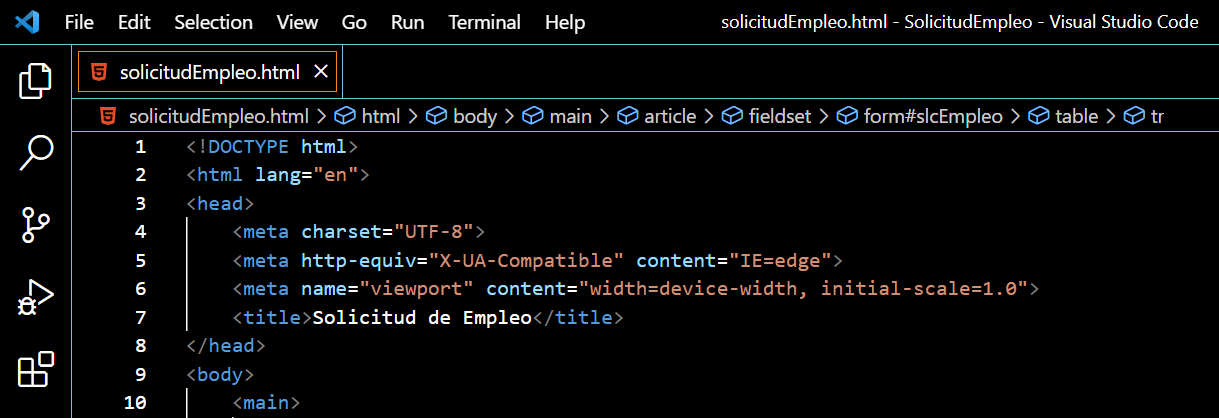
\includegraphics[scale=.54]{Capture}
	\centering
	\caption{Plantilla de VSC}
	\label{img:Capture}
\end{figure} 

Se definió como título "Solicitud de Empleo" y se empezó a codificar la página.

\begin{figure}[H]
	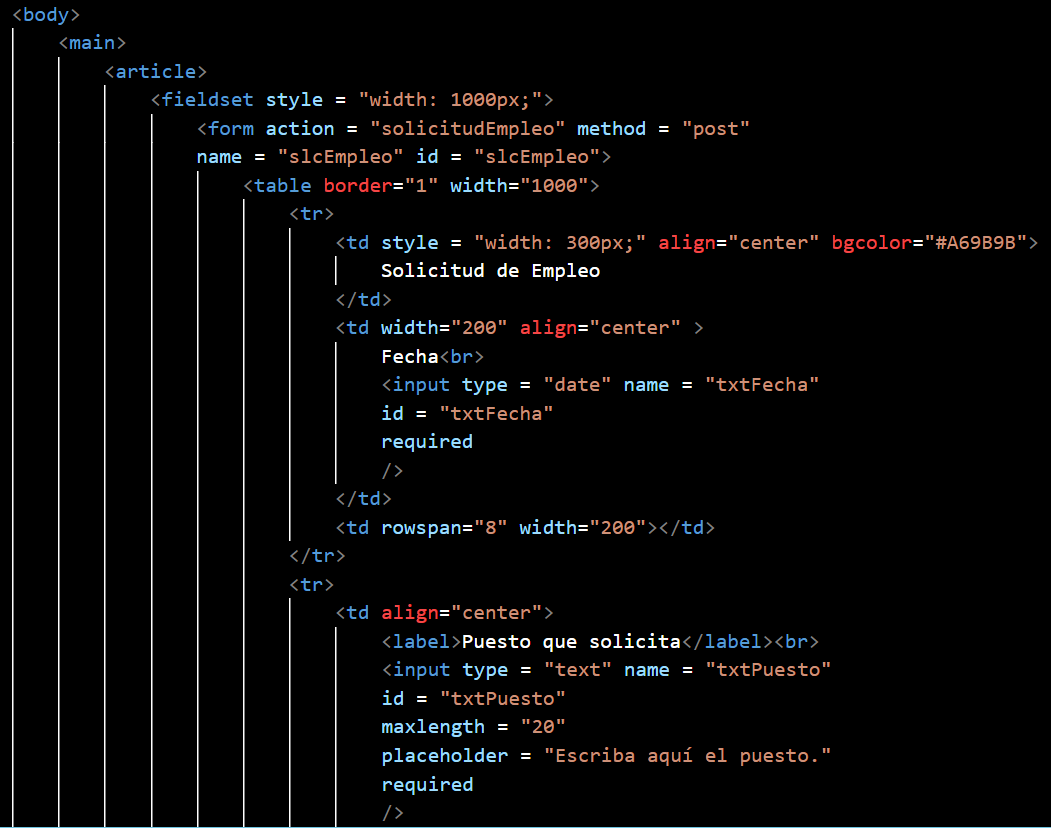
\includegraphics[scale=.54]{Capture2}
	\centering
	\caption{Fieldset, Formulario y Tabla}
	\label{img:Capture2}
\end{figure} 

Primero, se definió un fieldset de un ancho de 1000px, para que la información se viera de la mejor forma distribuida. Posteriormente, se creó un formulario con la instrucción form, donde se estableció como acción "solicitudEmpleo" y como método "POST". Estas dos características no se emplearon en este trabajo, pero sirven como muestra del funcionamiento de un formulario. De igual forma, se le adjuntó un id y name.

Luego, se inició la construcción de una tabla para una mayor facilidad de acomodo de toda la información requerida. Se le puso un borde de 1 y una anchura de 1000.

De esta forma, se pasó a definir todas sus filas, columnas y celdas. Para un mayor dinamismo a la hora de construir la solicitud, se decantó por realizar una tabla para cada apartado del documento. Asimismo, se emplearon distintas funcionalidades del input que se explicarán a continuación.

\subsection{
	\textit{
		\color{colorESCOM}{Funcionalidades del Formulario}
	}
}

Se emplearon siete herramientas para la creación del formulario, la mayoría con la instrucción input:

\begin{itemize}
	\item  text: Se le asignó a cada uno un id y name relacionado a lo requisitado en ese punto. También, se estableció en la mayoría una extensión máxima de 20, o hasta 50, carácteres con la instrucción maxlength; se pintó una oración de fondo en varios inputs para facilitar el saber que poner en cada uno de ellos con placeholder y se definió que fuera obligatorio el llenado de cada espacio con required.
	
	\begin{figure}[H]
		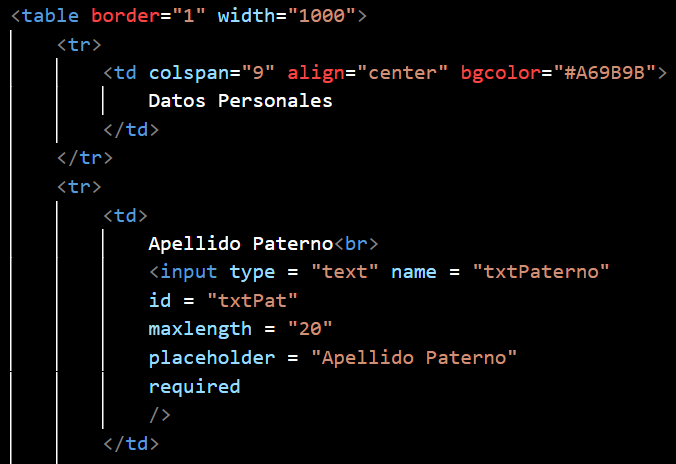
\includegraphics[scale=.54]{Capture4}
		\centering
		\caption{text}
		\label{img:Capture4}
	\end{figure} 
	
	\item  number: Ya definidos el id y name, se le dió una extensión máxima de 20 carácteres, un valor predefinido de 18 (value) y un rango entre 18 y 45 (min - max), haciendo caso a las reglas de negocio preestablecidas. Por último, se pidió que fuera obligatorio su llenado.
	
	\begin{figure}[H]
		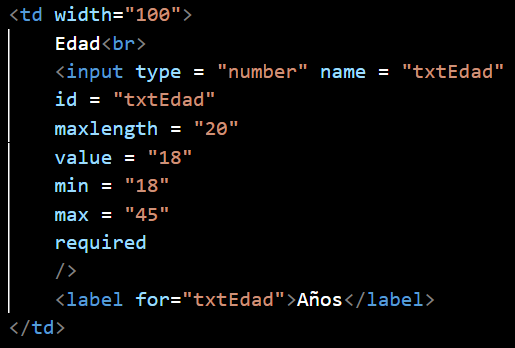
\includegraphics[scale=.54]{Capture5}
		\centering
		\caption{number}
		\label{img:Capture5}
	\end{figure} 
	
	\item  date: Sólamente se le asignó name, id y que fuera necesaria la elección de una fecha.
	
	\begin{figure}[H]
		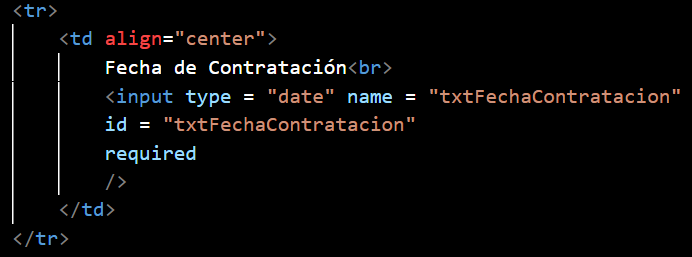
\includegraphics[scale=.54]{Capture3}
		\centering
		\caption{date}
		\label{img:Capture3}
	\end{figure} 
	
	\pagebreak	
	
	\item  radio: El uso de radio permite elegir entre un conjunto de opciones, sólo permitiendo quedarse con una. Se le asignó un name al conjunto de elecciones y un id diferente a cada uno. También, se le adjuntó un value por simple formalidad. Como característica adicional, se empleo la instrucción label para unir una palabra a cada radio.
	
	\begin{figure}[H]
		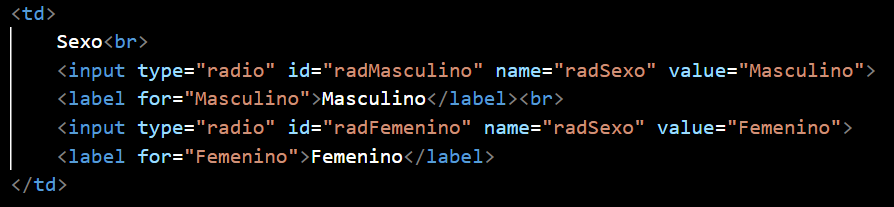
\includegraphics[scale=.54]{Capture6}
		\centering
		\caption{radio}
		\label{img:Capture6}
	\end{figure} 
	
	\item  checkbox: Muy parecido al radio, el tipo checkbox permite elegir varias opciones entre un conjunto de ellas. Se le asignó un name al grupo y un id individual. También, se escribió un value y el label para saber a que se refiere cada checkbox.
	
	\begin{figure}[H]
		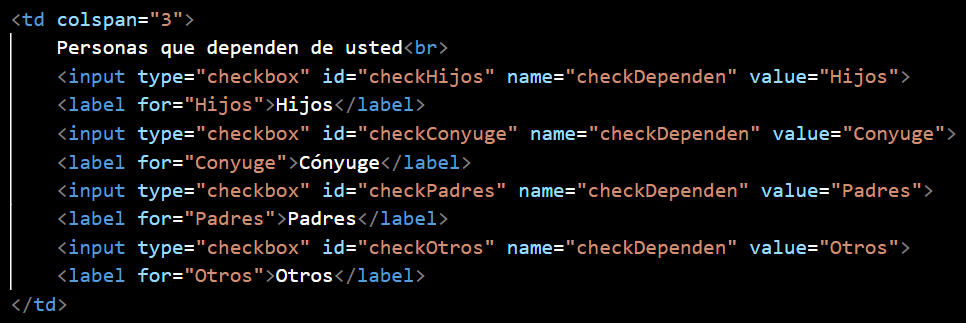
\includegraphics[scale=.54]{Capture7}
		\centering
		\caption{checkbox}
		\label{img:Capture7}
	\end{figure} 
	
	\item  textarea: Esta herramienta es un cuadro de texto, sólo que se puede modificar su tamaño. Se definió con 7 filas y 100 columnas por pura estética, aunque puede ser moldeado por el candidato. De igual modo, se le asignó un name.
	
	\begin{figure}[H]
		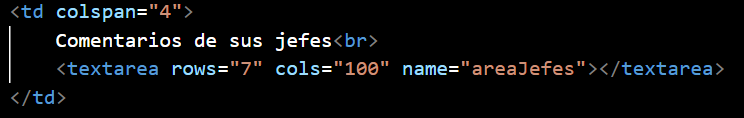
\includegraphics[scale=.54]{Capture9}
		\centering
		\caption{textarea}
		\label{img:Capture9}
	\end{figure} 
	
	\item  button (submit y reset): Con estas intrucciones, se puede crear botones que realizan distintas acciones. En el caso de submit, manda toda la información a la base de datos enlazada o al procesamiento requisitado (En esta práctica, no se trabajó en esa funcionalidad). En cuanto a reset, borra toda la información en cada uno de los apartados del formulario.
	
	\begin{figure}[H]
		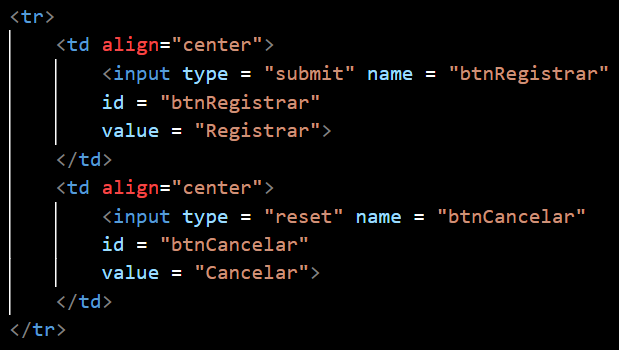
\includegraphics[scale=.54]{Capture8}
		\centering
		\caption{button. submit y reset}
		\label{img:Capture8}
	\end{figure} 
	
\end{itemize}

\subsection{
	\textit{
		\color{colorESCOM}{Funcionalidades de la Tabla}
	}
}

Con respecto a la tabla, más alla del uso de las filas y columnas, se empleó su capacidad de unir estas mismas con colspan y rowspan. Estas instrucciones fueron usadas cuanto fueron necesarias, de forma que se consiguiera el formato pedido.

\begin{figure}[H]
	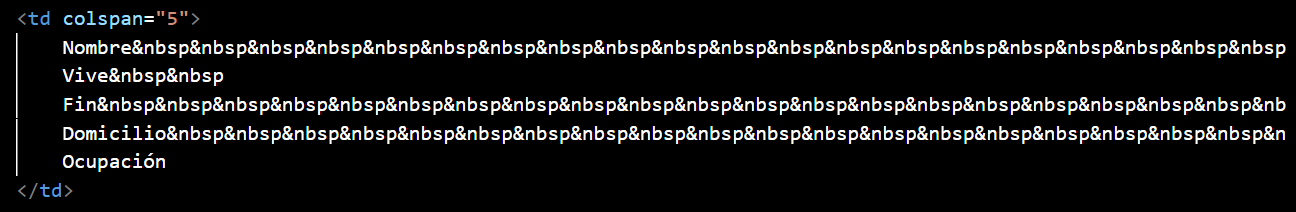
\includegraphics[scale=.54]{Capture11}
	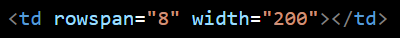
\includegraphics[scale=.54]{Capture12}
	\centering
	\caption{colspan y rowspan}
	\label{img:Capture12}
\end{figure} 

Asimismo, se emplearon nbsp y br para darle mayor estilo a la solicitud, al hacer espacios y saltos de línea, respectivamente.

\pagebreak

%################################################
\section{\color{colorIPN}{Resultados}}

Pasando a los resultado, se mostrará la página web y las distintas funcionalidades que provee, la cual se puede encontrar aquí: https://upbeat-swartz-2f3e65.netlify.app/.
%################################################
\subsection{	\color{colorESCOM}{Página Web}}

\begin{figure}[H]
	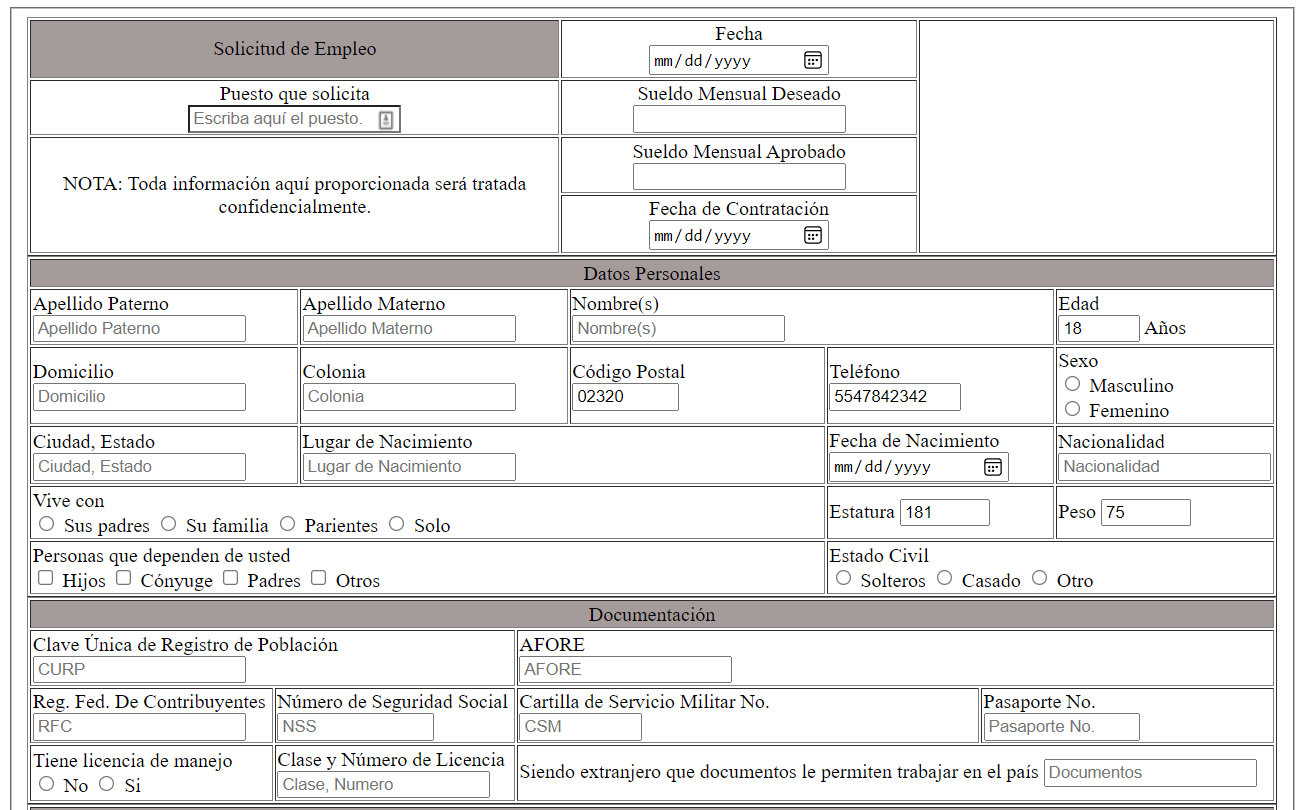
\includegraphics[scale=.54]{Capture10}
	\centering
	\caption{Funcionalidades}
	\label{img:Capture10}
\end{figure} 

En esta imagen, es posible observar la mayoría de funcionalidades comentadas en el apartado de desarrollo. Se tiene el fieldset y la separación en tablas por cuestión de estilo, el ingreso de datos por texto, número, fecha, radio y checkbox. Asimismo, esta el uso de colspan y rowspan para modificar la visibilidad de la información y el uso de bgcolor para sombrear ciertas celdas.

\begin{figure}[H]
	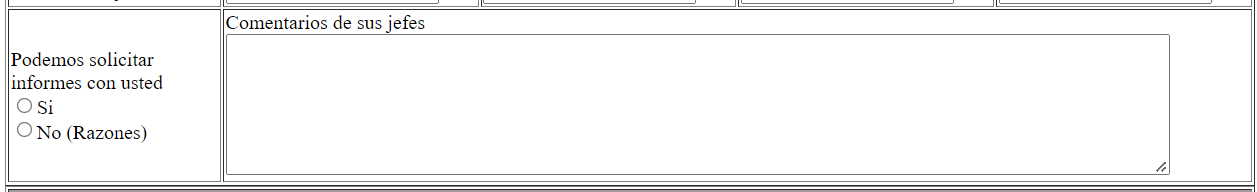
\includegraphics[scale=.54]{Capture13}
	\centering
	\caption{Funcionalidad. textarea}
	\label{img:Capture13}
\end{figure} 

\begin{figure}[H]
	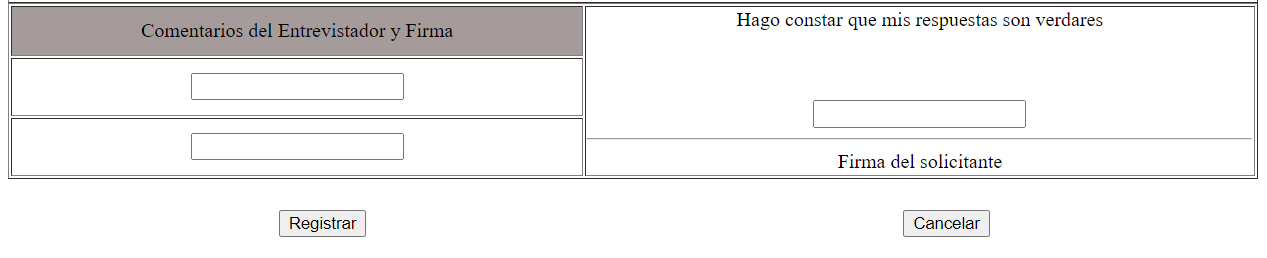
\includegraphics[scale=.54]{Capture14}
	\centering
	\caption{Funcionalidad. sumbit y reset}
	\label{img:Capture14}
\end{figure} 

Al igual, se tiene el textarea y los botones de registrar y cancelar.

\pagebreak

%################################################
\section{\color{colorIPN}{Conclusión}}
HTML es un lenguaje de hipertexto que abre varias posibilidades para crear páginas webs. Ciertamente, hoy en día ya hay tecnologías mucho más avanzadas para el desarrollo web, pero siempre es importante entender los principios de ciertas herramientas. Además, el trabajar con lo simple permite ir subiendo de dificultad poco a poco y solidificando cada vez más el conocimiento.

Considero que la práctica permite un aprendizaje prioritario y hace ver la estructura del código finamente.

\color{colorIPN}{
	\begin{flushright}
		\textit{
			Hurtado Morales Emiliano
		}
	\end{flushright} \hfill \break
}

\pagebreak

%################################################

\section{\color{colorIPN}{Referencias Bibliográficas}}
\color{colorESCOM}{
	\begin{thebibliography}{10}
		\bibitem[HTMLQuick]{HTMLQuick}
		De León, D.
		\newblock {\em Tablas en HTML}
		\newblock Recuperado el 4 de marzo de 2022, de https://www.htmlquick.com/es/tutorials/tables.html
	
		\bibitem[Conclase]{Conclase}
		Conclase
		\newblock {\em Formularios en documentos HTML}
		\newblock Recuperado el 4 de marzo de 2022, de http://html.conclase.net/w3c/html401-es/interact/forms.html
	
		\bibitem[OpenWebinars, 2019]{OpenWebinars}
		OpenWebinars
		\newblock {\em Que es HTML5}
		\newblock Recuperado el 4 de marzo de 2022, de https://openwebinars.net/blog/que-es-html5/
	\end{thebibliography}
}

\end{document}
